\subsection{Charging circuitry}
The LTC4425 is designed to charge a two ultra-capacitors in series from a USB port , forming a stack. It incorporates internal voltage clamp circuity to two present voltages, \SI{2.45}{V} or \SI{2.7}{V}, to prevent either of the ultra-capacitors from exceeding their maximum rated voltage. This clamping voltage can be configured externally and allowed flexibility for the ultra-capacitors chosen. It also allowed for an extra margin of safety for the \SI{2.7}{V} rated ultra-capacitors that were eventually chosen for the final design.
\\ \\
It was decided early on in the design process that a dedicated ultra-capacitor charge chip would be used rather than designing our own charging circuit using discrete components. This would free up a considerable amount of time that could then be used to design the rest of the hardware and fine tune the control algorithm.
\begin{figure}
    \centering
    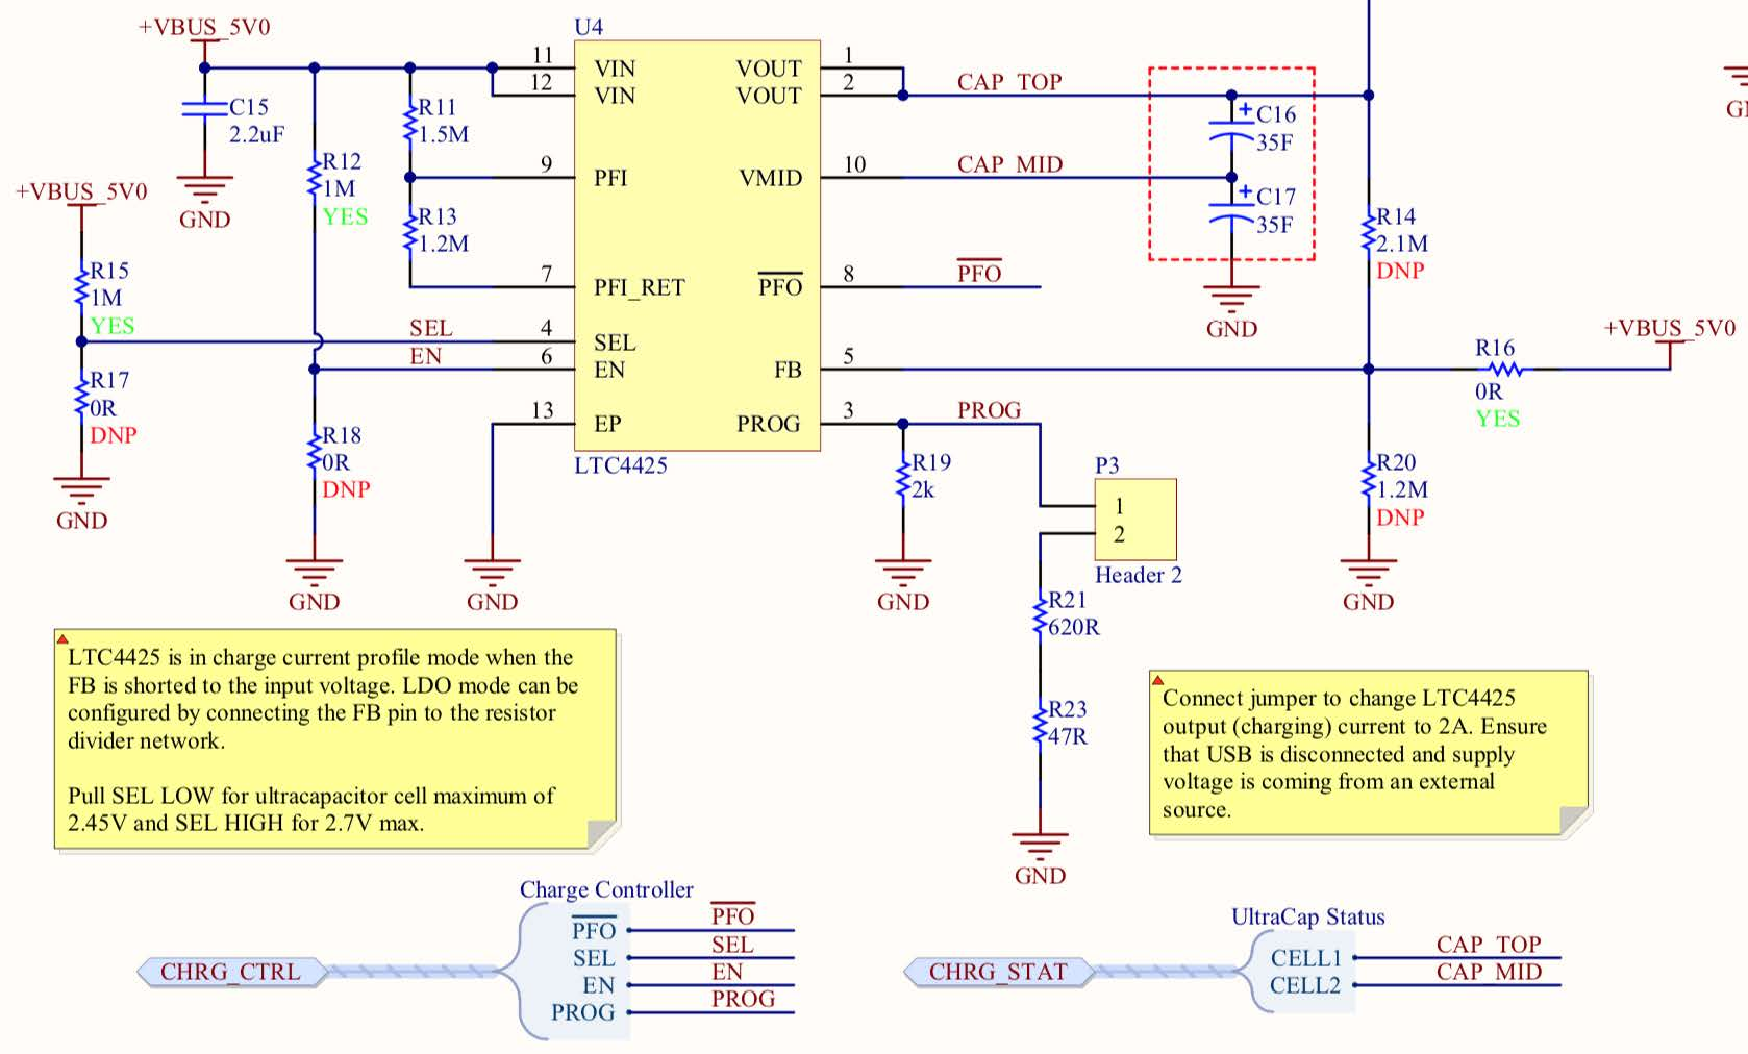
\includegraphics[height = 10cm]{figures/hardware/charging_schematic.pdf}
    \caption{Ultra-capacitor charging schematic excerpt.}
    \label{fig:charging}
\end{figure}
As capacitors appear as shorts to source voltages appearing across them that are higher than there currently stored voltage. Due to manufacturing tolerances the internal ESR of the capacitors can vary, this can lead to one of the capacitors sinking all the current, which causing one of the capacitors in the series stack to charge fully while the other does not. As the cell stack is being charged to \SI{5}{V} if one of the ultra-capacitors were to dominate it will lead to that capacitor being charged to \SI{5}{V}, well exceeding the specified \SI{2.7}{V} maximum leading to failure and potential explosion. To prevent this a charge balancing circuit is used that prevents the dominate cell from continuing to charge above the voltage of the other capacitor. By periodically preventing current flow the dominator cell, each ultra-capacitor can be charged to approximately the same potential. This could have been a complicated and time consuming analog circuit to implement in conjunction for this current limiter, therefore it was chosen to use an already designed charge management device that was designed for this purpose.
\\ \\
It was important that two ultra-capacitors were connected in series to allow for a larger operating rate and higher maximum voltage. This allows for the DC-DC converter to operate more efficiently at a significantly wider range of output values.

%%%%%%%%%%%%%%%%%%%%%%%%%%%%%%%%%%%%%%%%%%%%%%%%%%%%%%%%%%%%%%%%%%%%%%%%%%%%%%%%
\paragraph{LDO Mode}
Configuring the LTC4425 for LDO mode charges the top of the output capacitor to an externally programmed output voltage at a constant current, effectively operating as a low drop out regulator. To charge the ultra-capacitor stack from a USB port the constant current source is configured to \SI{500}{mA} such that the USB specification is met, in addition the output voltage is configured to be charged to \SI{5}{V}. To prevent the ultra-capacitors from an overvoltage condition, the charging voltage is clamped to a nominal \SI{2.7}{V} per cell, that is \SI{5.4}{V} across the entire stack. This is included to ensure that is the LTC4425 is configured in Normal Mode (where the output voltage charge to the within 7.5\% of the input voltage) or the FB resistors are incorrectly configured and the USB voltage is above the nominal \SI{5}{V} that it is specified to be.
\\ \\
The LDO mode resulted in the current being exceeded initially due to the effect of inrush current of a discharged capacitor. To prevent this the current limit was experimentally reduced to \SI{400}{mA}, in the future more robust current limiting circuitry would be included before the LTC4425.

%%%%%%%%%%%%%%%%%%%%%%%%%%%%%%%%%%%%%%%%%%%%%%%%%%%%%%%%%%%%%%%%%%%%%%%%%%%%%%%%

\paragraph{Charge Current Profile/Normal Mode}
To prevent inrush current (see below), the ultra-capacitors are charged initially at 10\% of the programmed current limit, providing \SI{50}{mA} charge current. It was found through experimentation that this worked well in preventing excessive current draw when the ultra-capacitors are completely discharged, however for the large capacitances used this proved to be too slow of a charging rate. Instead the LDO mode was chosen.
%%%%%%%%%%%%%%%%%%%%%%%%%%%%%%%%%%%%%%%%%%%%%%%%%%%%%%%%%%%%%%%%%%%%%%%%%%%%%%%%

\subsubsection{Ultra-capacitors}

%%%%%%%%%%%%%%%%%%%%%%%%%%%%%%%%%%%%%%%%%%%%%%%%%%%%%%%%%%%%%%%%%%%%%%%%%%%%%%%%

\paragraph{Inrush Current}
Connecting a source voltage to a capacitor which a potential difference smaller than that of the source will appear as a short circuit. It will draw current from the source as fast as it can, limited only by the internal resistance of the source and the ESR of the capacitor.

From start up, that is when the ultra-capacitors are completely discharged, the LTC4425 exceeds the current limit set by the Charge Current Program pin. When connected to a bench top power supply with a current limit set to \SI{500}{mA}, the output voltage sags as the current demand cannot be met. Increasing the current to limit to between \SI{560}-\SI{600}{mA} prevents this sagging, allowing the capacitors to charge. This overcurrent state last for a few seconds. If connected to a USB port this could potentially damage hardware.
\\ \\
%``The LTC4425 includes a soft-start circuit to minimize the inrush current at the start of a charge cycle. When a charge cycle is initiated, the charge current ramps from zero to full-scale over a period of approximately 1ms and this soft-start can be monitored by observing the PROG pin voltage. This has the effect of minimizing the transient current load on the power supply during start-up.'' \cite{ltc4425}